\chapter{成果呈現}
\label{chap:4}

本作业根据前面等章节所归纳出来的功能需求、技术方案、理论与模型等规划,同时检索现有的开放原始码项目,对现有的部分功能进行实作,当中完成的部分概念内容如下所示,其功能分别为学习检测、作业缴交、视频观看与教学直播。

\section{学习检测}

学习检测该功能为在视频观看与教学直播的功能下,由老师方或者管理方对学生们所发起的请求,当请求的当下学生可以接受或者拒绝,并且再给定的时间中进行分析并产生统计画面。下在面的测试则是尝试针对单一功能进行分析,检测目前做到单一次,但比需等待 3 秒左右的时间落差。其实际呈现如下图所示。该功能整合基于Python PyTorch 的 YOLOv5 模型、Python Flask 后端框架与 Node.js 的 Vue 前端框架为基础,对输入的画面进行分析来辨识画面中有没有人。

\begin{figure}[htb]
\centering 
\includegraphics[width=0.80\textwidth]{img/ch4m1.png} 
\caption{学习检测}
\label{Test}
\end{figure}

\section{作业缴交}

而作业缴交的功能则是研究 Python Flask  框架的特性,研究上传档案的机制后进行尝试。困难的地方在于再要求 Python Flask 后端框架对本地伺服器资源来操作档案时,必须要额外去写设定,从测试功能中可以看到档案可以上传到指定的目录下,之后规划可以为设定档案存档于伺服器某目录下,而后台资料库存放着该档案的路径。其画面如下所示。

\begin{figure}[htb]
\centering 
\includegraphics[width=0.80\textwidth]{img/demo-file-sys-0.png} 
\caption{作业缴交选择档案}
\label{Test}
\end{figure}

\begin{figure}[htb]
\centering 
\includegraphics[width=0.80\textwidth]{img/demo-file-sys-1.png} 
\caption{作业缴交的选择状态}
\label{Test}
\end{figure}

\section{视频观看与聊天讨论功能}

此功能则是研究 Python Flask 框架的特性,预设播放视频需要特别去设定,同时本地端汇入 JS 与 CSS 插件,则有着额外的写法,另外聊天室的部分则在此使用 Socket.io 与 Web Socket 进行处理。两部分如下所示。当中视频观看功能则可以将显示的时间进行回传。

\begin{figure}[htb]
\centering 
\includegraphics[width=0.80\textwidth]{img/demo-chat-sys.png} 
\caption{聊天讨论功能}
\label{Test}
\end{figure}

\begin{figure}[htb]
\centering 
\includegraphics[width=0.80\textwidth]{img/demo-video-sys.png} 
\caption{视频观看}
\label{Test}
\end{figure}

\section{教学直播}

此功能则是研究 Python Flask 框架与 OpenCV 特性,该功能初期研究过目前的串流服务,并在本地的伺服器端考量 FFMPEG 进行处理。从测试画面中可以看到人脸辨识的画面。该测试测试功能目标在于进行串流时,辨识出人脸。未来计画与学习检测进行整合。

\begin{figure}[htb]
\centering 
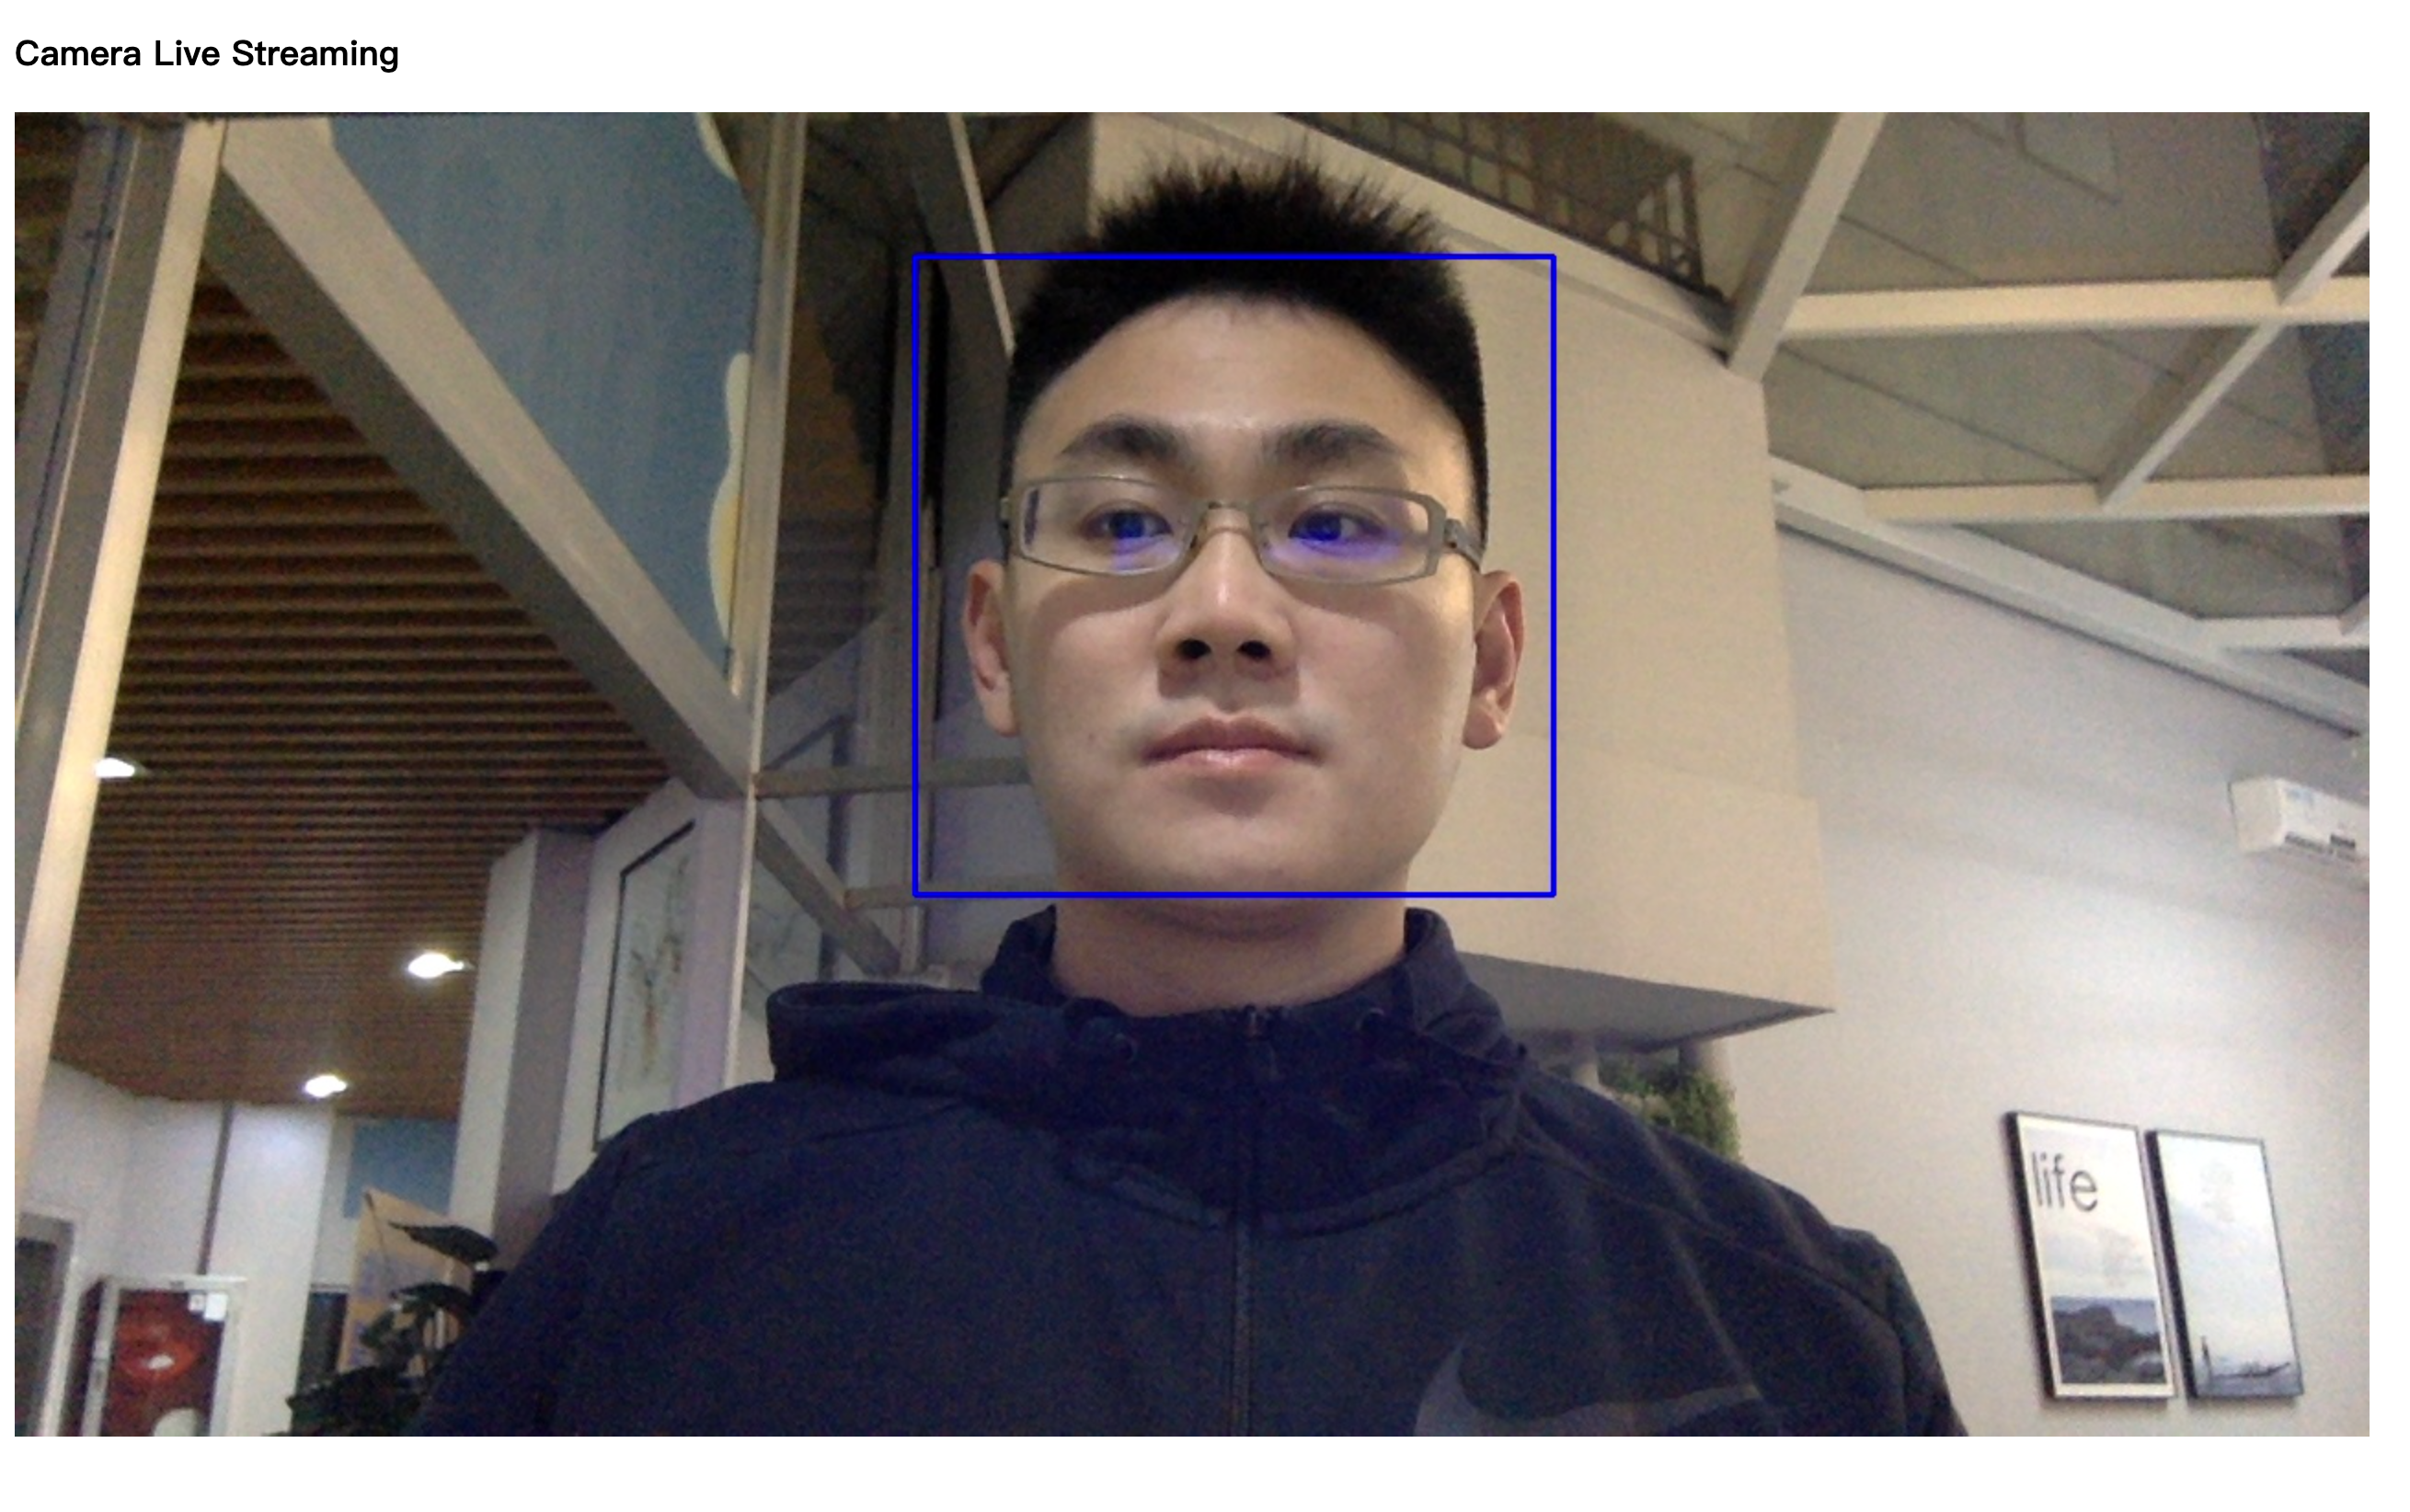
\includegraphics[width=0.80\textwidth]{img/demo-streaming-sys.png} 
\caption{教学直播}
\label{Test}
\end{figure}
